% Problem 21
\Needspace{18\baselineskip}
\item \label{prob:21}
A student wants to set up an experiment with a thin convex lens of focal length $f$ such that a thin real object produces a focused real image on a movable screen. At how many locations along the optical axis can the object be placed so that the distance between the object and the focused image on the screen is equal to $3f$?
\begin{enumerate}[label=(\Alph*)]
    \item There is no location.
    \item There is exactly one location.
    \item There are exactly two locations.
    \item There are exactly four locations.
    \item There are an infinite number of locations.
\end{enumerate}

\category{Geometric Optics}
\StudyGuideLinks{21}
\ProblemSource{21}
\begin{answerbox}
\finalanswer{(A) There is no location.}
\end{answerbox}
\begin{insightbox}
Solve $1/d_o+1/d_i=1/f$ with $d_o+d_i=3f$; the quadratic has negative discriminant, so no real location. Only when the object–image separation $D\ge 4f$ can a real solution exist.
\end{insightbox}
\begin{solutionbox}

With $\tfrac{1}{d_o}+\tfrac{1}{d_i}=\tfrac{1}{f}$ and $D=d_o+d_i=3f$, substitute $d_i=3f-d_o$:
\[
\frac{1}{d_o}+\frac{1}{3f-d_o}=\frac{1}{f} \Rightarrow d_o^2-3fd_o+3f^2=0.
\]
Discriminant $\Delta=9f^2-12f^2=-3f^2<0$, so no real $d_o$ exists.
\end{solutionbox}

% Problem 22
\Needspace{18\baselineskip}
\item \label{prob:22}
\noindent\begin{minipage}[t]{0.6\linewidth}
\vspace{0pt}
For the circuit shown, all wires have no resistance, the battery has a constant internal resistance of $r = 8.0\,\Omega$ and the two light bulbs are identical. The variable resistor is initially set to $R = 26.0\,\Omega$. The switch S is closed. To what resistance must the variable resistor be set if bulb \#1 is to have the same brightness after the switch is closed as it did with the switch open?
\begin{enumerate}[label=(\Alph*)]
    \item $9.0\,\Omega$
    \item $13.0\,\Omega$
    \item $18.0\,\Omega$
    \item $22.0\,\Omega$
    \item The answer can be computed only if the bulbs’ resistance is known.
\end{enumerate}
\end{minipage}%
\hfill
\begin{minipage}[t]{0.32\linewidth}
\vspace{0pt}
\centering
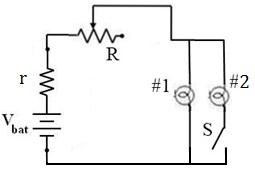
\includegraphics[width=\linewidth]{Problem_21_Figure.png}
\end{minipage}

\category{DC Circuits}
\StudyGuideLinks{22}
\ProblemSource{22}
\begin{answerbox}
\finalanswer{(A) $9.0\,\Omega$}
\end{answerbox}
\begin{insightbox}
Keep bulb 1 current unchanged; equate open/closed currents in the equivalent circuits to solve $R'$.
\end{insightbox}
\begin{solutionbox}

Open: $I_{1,\text{open}}=\tfrac{\mathcal E}{r+R_b+R}$. Closed: bulbs in parallel $R_p=R_b/2$, total $r+R_b/2+R'$, current splits equally so $I_{1,\text{closed}}=\tfrac{\mathcal E}{2r+R_b+2R'}$. Equate:
\[
r+R_b+R=2r+R_b+2R' \Rightarrow R' = \tfrac{R-r}{2} = \tfrac{26-8}{2}=9.0\,\Omega.
\]
\end{solutionbox}

% Problem 23
\Needspace{18\baselineskip}
\item \label{prob:23}
\noindent\begin{minipage}[t]{0.6\linewidth}
\vspace{0pt}
A mass on a frictionless incline has a gravitational force, a normal force, and an applied force that all are equal in magnitude. The mass remains at rest. The incline makes an angle $\theta$ with the horizontal. Which one of the following choices best describes the orientation of the applied force? The +x-axis is parallel to the incline’s surface.
\begin{enumerate}[label=(\Alph*)]
    \item Oriented directly along the +x axis.
    \item Oriented at an angle $\theta$ clockwise from the +x axis.
    \item Oriented at an angle $90^\circ - \theta$ clockwise from the +x axis.
    \item Oriented at an angle $90^\circ - \theta$ counterclockwise from the +x axis.
    \item This is a completely impossible situation.
\end{enumerate}
\end{minipage}%
\hfill
\begin{minipage}[t]{0.32\linewidth}
\vspace{0pt}
\centering
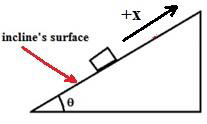
\includegraphics[width=\linewidth]{Problem_23_Figure.png}
\end{minipage}

\category{Statics}
\StudyGuideLinks{23}
\ProblemSource{23}
\begin{answerbox}
\finalanswer{(C) Oriented at $90^\circ-\theta$ clockwise from +x}
\end{answerbox}
\begin{insightbox}
Resolve the applied force along and perpendicular to the incline, then use its given magnitude.
\end{insightbox}
\begin{solutionbox}
The force components needed for equilibrium are $F_{a,x}=mg\sin\theta$ and $F_{a,y}=mg(\cos\theta-1)$. Since $F_a=mg$, their squared magnitudes give $2(1-\cos\theta)=1$, hence $\theta=60^\circ$ for an incline. The applied force is therefore $30^\circ=90^\circ-\theta$ clockwise from the $+x$ axis. The stated equal-force condition itself fixes the incline angle.
\end{solutionbox}

% Problem 24
\Needspace{18\baselineskip}
\item \label{prob:24}
The position of a mass connected to a spring obeys $x(t) = A \cos(\omega t)$. What is the average speed of the mass for one full oscillation in terms of the mass’s maximum speed during oscillation, $v_{max}$?
\begin{enumerate}[label=(\Alph*)]
    \item $\frac{2}{\pi} v_{max}$
    \item $\frac{1}{\sqrt{2}} v_{max}$
    \item $\frac{1}{2} v_{max}$
    \item $\frac{\sqrt{2}}{\pi} v_{max}$
    \item $\frac{1}{2\pi\sqrt{2}} v_{max}$
\end{enumerate}

\category{Oscillations}
\StudyGuideLinks{24}
\ProblemSource{24}
\begin{answerbox}
\finalanswer{(A) $\tfrac{2}{\pi}v_{max}$}
\end{answerbox}
\begin{insightbox}
In one period distance is $4A$, $T=2\pi/\omega$, and $v_{max}=A\omega$; substitute to get $\bar s=(2/\pi)v_{max}$.
\end{insightbox}
\begin{solutionbox}

During one period $T=2\pi/\omega$, distance covered is $4A$. With $v_{max}=A\omega$, the average speed is $\bar s=4A/T=2A\omega/\pi=\tfrac{2}{\pi}v_{max}$.
\end{solutionbox}

% Problem 25
\Needspace{18\baselineskip}
\item \label{prob:25}
\noindent\begin{minipage}[t]{0.6\linewidth}
\vspace{0pt}
An upward-pointing object is placed 15.0 cm to the left of a lens system. The first lens is convex with focal length 10.0 cm. The second lens is convex with focal length 10 cm and its location from the first lens is varied from $x=10$ cm away to $x=110$ cm away. Which one of the following choices best represents the description of the final image formed as the second lens is moved from $x=10$ cm to $x=110$ cm from the first lens?
\end{minipage}%
\hfill
\begin{minipage}[t]{0.32\linewidth}
\vspace{0pt}
\centering
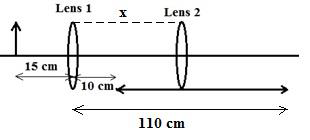
\includegraphics[width=\linewidth]{Problem_26_Figure.png}
\end{minipage}

\begin{enumerate}[label=(\Alph*)]
    \item $x=10$ cm away: Real \& pointing downward; $\quad x=110$ cm away: Real \& pointing upward
    \item $x=10$ cm away: Virtual \& pointing downward; $\quad x=110$ cm away: Real \& pointing upward
    \item $x=10$ cm away: Virtual \& pointing upward; $\quad x=110$ cm away: Real \& pointing downward
    \item $x=10$ cm away: Real \& pointing upward; $\quad x=110$ cm away: Real \& pointing upward
    \item $x=10$ cm away: Virtual \& pointing downward; $\quad x=110$ cm away: Virtual \& pointing downward
\end{enumerate}

\category{Geometric Optics}
\StudyGuideLinks{25}
\ProblemSource{25}
\begin{answerbox}
\finalanswer{(A) Real \& pointing downward at $x=10$ cm; Real \& pointing upward at $x=110$ cm.}
\end{answerbox}
\begin{insightbox}
The image of the first lens is the object for the second; its signed distance changes as the second lens moves.
\end{insightbox}
\begin{solutionbox}
\textbf{Behavior vs. $x$:} The final image is real and inverted for $10\le x<30$, becomes virtual and inverted for $30<x<40$, and is real and upright for $x>40$. At $x=30$ the intermediate image lies in the second lens plane, so the usual object-distance formula is singular; at $x=40$ the image lies at infinity.

Using $d_{i1}=30\,\text{cm}$ from lens 1, the second lens has $d_{o2}=x-30$. With $f_2=10$ cm,
\[ d_{i2}=\frac{10(x-30)}{x-40}, \quad m_{\text{total}}=\frac{20}{x-40}. \]
Signs of $d_{i2}$ and $m_{\text{total}}$ across intervals give the stated behavior.
\end{solutionbox}

% Problem 26
\Needspace{18\baselineskip}
\item \label{prob:26}
Rain falls vertically at 12.0 m/s in the ground frame. A car travels down a slope at $40^\circ$ below the horizontal. A passenger sees the rain moving at $29.0^\circ$ from vertical. What is the car's speed relative to the ground?
\begin{enumerate}[label=(\Alph*)]
    \item 2.29 m/s
    \item 5.93 m/s
    \item 9.03 m/s
    \item 11.8 m/s
    \item 16.2 m/s
\end{enumerate}

\category{Relative Motion}
\StudyGuideLinks{26}
\ProblemSource{26}
\begin{answerbox}
\finalanswer{(B) $5.93\,\text{m/s}$}
\end{answerbox}
\begin{insightbox}
Subtract the car's velocity from the rain's velocity in both horizontal and vertical components.
\end{insightbox}
\begin{solutionbox}

Take right and up as positive. The rain has $\vec v_{r/g}=(0,-12)$ and the car has $\vec v_{c/g}=(v_c\cos40^\circ,-v_c\sin40^\circ)$. Thus $\vec v_{r/c}=(-v_c\cos40^\circ,-12+v_c\sin40^\circ)$. The passenger's observation gives
\[
\tan29^\circ=\frac{v_c\cos40^\circ}{12-v_c\sin40^\circ}
\quad\Rightarrow\quad
v_c=\frac{12\tan29^\circ}{\cos40^\circ+\sin40^\circ\tan29^\circ}
\approx5.93\,\mathrm{m/s}.
\]
\emph{Editorial note:} The earlier repository transcription contained conflicting directions. The slope and $29^\circ$ observation above follow the original 2015 problem.
\end{solutionbox}

% Problem 27
\Needspace{18\baselineskip}
\item \label{prob:27}
\noindent\begin{minipage}[t]{0.6\linewidth}
\vspace{0pt}
A 2.0 kg mass is connected to the end of string and moves about the string’s fixed end in a conical motion with a constant speed of 4.0 m/s. The string has a length of 2.50 m and forms an angle of $\theta$ with the vertical. Use $g=10\,\mathrm{m/s^2}$. What is the tension in the string?
\begin{enumerate}[label=(\Alph*)]
    \item 20.0 N
    \item 23.7 N
    \item 27.4 N
    \item 29.8 N
    \item 32.5 N
\end{enumerate}
\end{minipage}%
\hfill
\begin{minipage}[t]{0.35\linewidth}
\vspace{0pt}
\centering
\begin{tikzpicture}[scale=0.95,>=Stealth]
  \coordinate (pivot) at (0,2);
  \coordinate (mass) at (1.2,0);
  \draw[dashed] (pivot) -- (0,0) -- (mass);
  \draw[thick] (pivot) -- (mass) node[midway,right] {$L$};
  \fill (pivot) circle (1.5pt);
  \filldraw[fill=blue!15] (mass) circle (3pt) node[right=4pt] {$m$};
  \draw (0,1.5) arc[start angle=-90,end angle=-59,radius=.5];
  \node at (.23,1.25) {$\theta$};
  \node[right] at (1.38,.16) {$\vec v:\odot$};
\end{tikzpicture}
\end{minipage}

\category{Circular Motion}
\StudyGuideLinks{27}
\ProblemSource{27}
\begin{answerbox}
\finalanswer{(C) 27.4 N}
\end{answerbox}
\begin{insightbox}
Use vertical equilibrium and horizontal centripetal acceleration, with the circular radius $r=L\sin\theta$.
\end{insightbox}
\begin{solutionbox}

From $T\cos\theta=mg$ and $T\sin\theta=mv^2/(L\sin\theta)$, eliminate $\theta$:
\[
 T-\frac{(mg)^2}{T}=\frac{mv^2}{L}=12.8\,\mathrm N.
\]
The positive root of $T^2-12.8T-400=0$ is $T\approx27.4\,\mathrm N$.
\end{solutionbox}

% Problem 28
\Needspace{18\baselineskip}
\item \label{prob:28}
\noindent\begin{minipage}[t]{0.6\linewidth}
\vspace{0pt}
A box slides with uniform acceleration up an incline. The box has an initial speed of 9.0 m/s and rises vertically 2.60 m before coming to rest. Use $g=10\,\mathrm{m/s^2}$. If the angle of the incline is $30^\circ$, what is the coefficient of kinetic friction between the box and the incline?
\begin{enumerate}[label=(\Alph*)]
    \item 0.298
    \item 0.322
    \item 0.372
    \item 0.483
    \item 0.557
\end{enumerate}
\end{minipage}%
\hfill
\begin{minipage}[t]{0.35\linewidth}
\vspace{0pt}
\centering
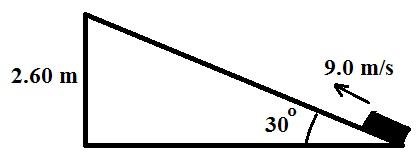
\includegraphics[width=\linewidth]{Problem_28_Figure.png}
\end{minipage}

\category{Work \& Energy with Friction}
\StudyGuideLinks{28}
\ProblemSource{28}
\begin{answerbox}
\finalanswer{(B) 0.322}
\end{answerbox}
\begin{insightbox}
The initial kinetic energy becomes gravitational potential energy and thermal energy from friction.
\end{insightbox}
\begin{solutionbox}

Energy lost to friction is positive on the right-hand side:
\[
\tfrac12 mv^2=mgh+\mu_k mg\cos30^\circ\,d,
\qquad d=\frac{2.60}{\sin30^\circ}=5.20\,\mathrm m.
\]
Therefore $\mu_k=(40.5-26.0)/(10\cos30^\circ\cdot5.20)\approx0.322$.
\end{solutionbox}

% Problem 29
\Needspace{18\baselineskip}
\item \label{prob:29}
\noindent\begin{minipage}[t]{0.6\linewidth}
\vspace{0pt}
A 9.20 m long uniform plank rests on a frictionless ice pond. A 52 kg box rests on the plank’s left end while a 71 kg person stands at the plank’s right end. After the person walks to the left on the plank and stands at the same location as the box, the plank has slid 3.84 m to the right relative to the pond’s shore. Which one of the following choices best represents the mass of the plank?
\begin{enumerate}[label=(\Alph*)]
    \item 123 kg
    \item 61.5 kg
    \item 47.1 kg
    \item 36.5 kg
    \item 31.2 kg
\end{enumerate}
\end{minipage}%
\hfill
\begin{minipage}[t]{0.35\linewidth}
\vspace{0pt}
\centering
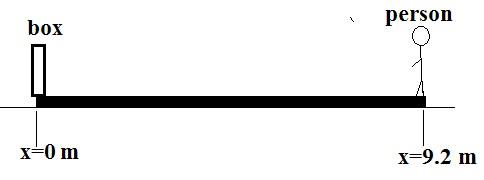
\includegraphics[width=\linewidth]{Problem_29_Figure.png}
\end{minipage}

\category{Center of Mass}
\StudyGuideLinks{29}
\ProblemSource{29}
\begin{answerbox}
\finalanswer{(C) 47.1 kg}
\end{answerbox}
\begin{insightbox}
No external horizontal force acts, so the horizontal center of mass remains fixed.
\end{insightbox}
\begin{solutionbox}

Stationary center of mass: $M_p\Delta x_p+M_b\Delta x_b+M_{pers}\Delta x_{pers}=0$. With given displacements, $3.84M_p+199.68-380.56=0 \Rightarrow M_p\approx47.1\,\text{kg}$.
\end{solutionbox}

% Problem 30
\Needspace{18\baselineskip}
\item \label{prob:30}
At the top of a high cliff, a small rock is dropped from rest. A ball is launched straight downward with an initial speed of 36.0 m/s at a time of 2.10 s after the rock was dropped. Use $g=10\,\mathrm{m/s^2}$. When the ball has fallen 28.0 m further than the initially dropped rock, what is the speed of the ball relative to the rock?
\begin{enumerate}[label=(\Alph*)]
    \item 15.0 m/s
    \item 16.0 m/s
    \item 20.0 m/s
    \item 21.0 m/s
    \item 36.0 m/s
\end{enumerate}

\category{Kinematics}
\StudyGuideLinks{30}
\ProblemSource{30}
\begin{answerbox}
\finalanswer{(A) 15.0 m/s}
\end{answerbox}
\begin{insightbox}
Once both objects are in flight their accelerations match, so their relative velocity is constant.
\end{insightbox}
\begin{solutionbox}

Downward speeds: $v_r=gt$, $v_b=36+g(t-2.10)$ for $t\ge2.10$. Relative speed $v_{rel}=v_b-v_r=36-g\cdot2.10\approx15.0\,\text{m/s}$ (using $g\approx10\,\text{m/s}^2$).
\end{solutionbox}
